\chapter[Proposta]{Proposta}
\label{sec:proposta}

\section{Metodologia}
\label{sec:metodologia}

\subsection{Metodologia de Pesquisa}

\subsubsection{Quanto à abordagem}

Em relação à abordagem qualitativa, esta se caracteriza por um enfoque interpretativo e subjetivo, voltado para a compreensão aprofundada dos fenômenos em estudo. Tal abordagem visa descrever e interpretar a complexidade das relações sociais, compreendendo as significações atribuídas pelos indivíduos às suas experiências e práticas. Diferentemente da abordagem quantitativa, que busca generalizações a partir de dados numéricos, a qualitativa concentra-se na riqueza dos detalhes e na profundidade da análise, sendo especialmente eficaz em contextos onde é necessário entender processos, motivações e interações sociais intrínsecas ao objeto de estudo, de acordo com o quadro teórico-metodológico proposto por \cite{Gerhardt2009}.

O principal objetivo, como mencionado na seção \ref{sec:objetivos} deste trabalho é desenvolver um software educativo em português voltado para os sistemas operacionais Linux e Windows, proporcionando um ambiente simples e intuitivo para o aprendizado das estruturas básicas do SQL. Para alcançar esse objetivo, é essencial compreender as dificuldades enfrentadas por estudantes na aprendizagem dessa linguagem, o que exige uma abordagem qualitativa que explore as barreiras e fatores que afetam a compreensão da linguagem.

\subsubsection{Quanto à natureza}

O presente trabalho, ao se concentrar no desenvolvimento de um software destinado a auxiliar estudantes iniciantes em bancos de dados relacionais, sendo assim, classifica-se como uma pesquisa de natureza aplicada, uma vez que visa abordar e solucionar um problema.\cite{Gerhardt2009} 


\subsubsection{Quanto aos objetivos}

A pesquisa exploratória tem como finalidade aprofundar a compreensão do problema investigado, tornando-o mais claro e permitindo a formulação de hipóteses. Esse tipo de pesquisa geralmente envolve a realização de um levantamento bibliográfico que auxilie na compreensão do contexto.\cite{Gerhardt2009}

Esta pesquisa pode ser classificado como exploratória, uma vez que foi realizado um levantamento de informações pertinentes por meio de uma pesquisa bibliográfica, conforme descrito no Capítulo \ref{sec:referencial}. Essa abordagem visa esclarecer o problema em estudo e possibilitar a formulação de hipóteses fundamentadas. Assim, a pesquisa exploratória contribui para uma compreensão mais abrangente do tema investigado.



\subsubsection{Quanto aos Procedimentos}

A pesquisa bibliográfica é um procedimento essencial na investigação científica que consiste no levantamento de referências teóricas previamente analisadas visando reunir informações e conhecimentos prévios que ajudem a esclarecer o problema em questão \cite{Gerhardt2009}. Em consonância com esse procedimento, este trabalho reuniu informações no Capítulo \ref{sec:referencial}.

A produção tecnológica é entendida como um conjunto de processos e produtos que visam solucionar problemas práticos e atender às necessidades da sociedade, contribuindo para o desenvolvimento tecnológico, econômico e social \cite{Serzedello_Tomael_2011}.

\subsection{Cronograma}
\label{sec:cronograma}

A Tabela \ref{tab:cronograma_tcc1} apresenta o cronograma detalhado das atividades planejadas para a realização do TCC1, organizando-as ao longo dos meses. As etapas iniciais focam na definição do escopo do trabalho, envolvendo a escolha da área de pesquisa e a discussão com o orientador sobre possibilidades, culminando na escolha e validação de um tema alinhado às expectativas das partes envolvidas. Essas ações são fundamentais para estabelecer as bases do projeto e garantir sua relevância acadêmica.

Posteriormente, o cronograma direciona-se para a execução prática do trabalho. Isso inclui desde a elaboração da introdução e a pesquisa bibliográfica, que fornecem o contexto teórico necessário, até o desenvolvimento e revisão de uma proposta de solução. As etapas finais abrangem a correção de problemas apontados pelo orientador, a redação das considerações finais e, por fim, a apresentação do TCC1 à banca avaliadora.

\begin{table}[h!]
    \centering
    \begin{tabular}{|m{6cm}|c|c|c|c|c|}
        \hline
        \textbf{Atividade} & \textbf{Out} & \textbf{Nov} & \textbf{Dez} & \textbf{Jan} & \textbf{Fev} \\ \hline
        Discutir com o orientador sobre a área do tema & X & X & & & \\ \hline
        Definir tema & & X & & & \\ \hline
        Validar com o Orientador & & X & & & \\ \hline
        Escrever a introdução & & X &  & & \\ \hline
        Realizar pesquisa bibliográfica & & & X & X &  \\ \hline
        Elaborar proposta de solução & & & & X & \\ \hline
        Escrever considerações finais & & & & X &  \\ \hline
        Corrigir problemas apontados pelo orientador & & & & X & X \\ \hline
        Apresentar TCC1 para banca & & & & & X \\ \hline
    \end{tabular}
    \caption{Cronograma de Atividades TCC1.}
    \label{tab:cronograma_tcc1}
    Fonte: Autoria própria.
\end{table}

\subsection{Metodologia de Desenvolvimento de Software}
\label{sec:metodologia_de_desenvolvimento_de_software}

\subsubsection{Extreme Programming (XP)}

Extreme Programming (XP) é uma metodologia ágil que visa melhorar a qualidade do software e a capacidade de resposta às mudanças dos requisitos dos clientes. XP é caracterizado por um conjunto de valores, princípios e práticas que promovem a comunicação eficaz, a simplicidade no design e a adaptação constante ao feedback \cite{beckKent2004}.

\subsubsubsection{Valores}

A metodologia de Extreme Programming é centrada em quatro valores fundamentais, dos quais destacam-se nesse projeto a simplicidade e a coragem \cite{beckKent2004}. 

A simplicidade, como valor, busca minimizar a complexidade do desenvolvimento, incentivando a criação do sistema mais simples possível que atenda aos requisitos atuais. Ressalta-se que um design simples não apenas facilita a manutenção e a extensão do sistema, mas também reduz os custos e o tempo de desenvolvimento \cite{beckKent2004}.

A coragem, por sua vez, é necessária para enfrentar mudanças e dificuldades, incentivando os desenvolvedores a refatorar o código e a eliminar recursos desnecessários sem medo de comprometer o projeto em andamento \cite{beckKent2004}.

\subsubsubsection{Princípios}

Além dos valores, XP é guiado por princípios, dos quais a qualidade e os \textit{baby steps} são centrais para esse projeto. 

O princípio da qualidade, \cite{beckKent2004} enfatiza a importância de entregar um software que atenda aos requisitos de funcionalidade e confiabilidade. 

A abordagem de \textit{baby steps}, ou passos pequenos, sustenta que a implementação de mudanças deve ser feita de forma incremental e iterativa, permitindo um constante ajuste e refinamento do sistema sem a introdução de grandes riscos ou rupturas \cite{beckKent2004}.

\subsubsubsection{Práticas}

As práticas de XP são estruturadas para suportar seus valores e princípios, e incluem o \textit{Weekly Cycle} e o \textit{Incremental Design}. 

O \textit{Weekly Cycle} consiste em ciclos de desenvolvimento semanais, nos quais o progresso é revisado e novos planos são estabelecidos. Esta prática promove a adaptação rápida às mudanças de requisitos. Já o \textit{Incremental Design} é uma abordagem que defende a evolução contínua do design do sistema, permitindo que ele cresça e se adapte conforme novas funcionalidades são integradas \cite{beckKent2004}.

Durante as reuniões semanais, é necessário revisar não apenas o progresso realizado, mas também identificar e planejar as próximas histórias a serem implementadas, garantindo que o foco esteja sempre na entrega incremental de valor.

\section{Requisitos}

\section{Arquitetura}

\section{Suporte Tecnológico}

\subsection{Git}

O Git é um sistema de controle de versão distribuído, amplamente utilizado no desenvolvimento de software para rastrear alterações no código-fonte durante o desenvolvimento de projetos. Git se destaca por sua eficiência e velocidade, permitindo que desenvolvedores trabalhem de forma colaborativa e independente em diferentes partes de um projeto \cite{git2025}.

A figura \ref{fig:git2025} ilustra um modelo de desenvolvimento distribuído, onde vários \textit{developers} colaboram por meio de um repositório compartilhado, denominado \textit{shared repository}. Cada \textit{developer} tem a capacidade de contribuir, realizar alterações e sincronizar com o repositório, permitindo uma colaboração eficiente e um fluxo de trabalho integrado \cite{git2025}.

\begin{figure}[h!]
    \centering
    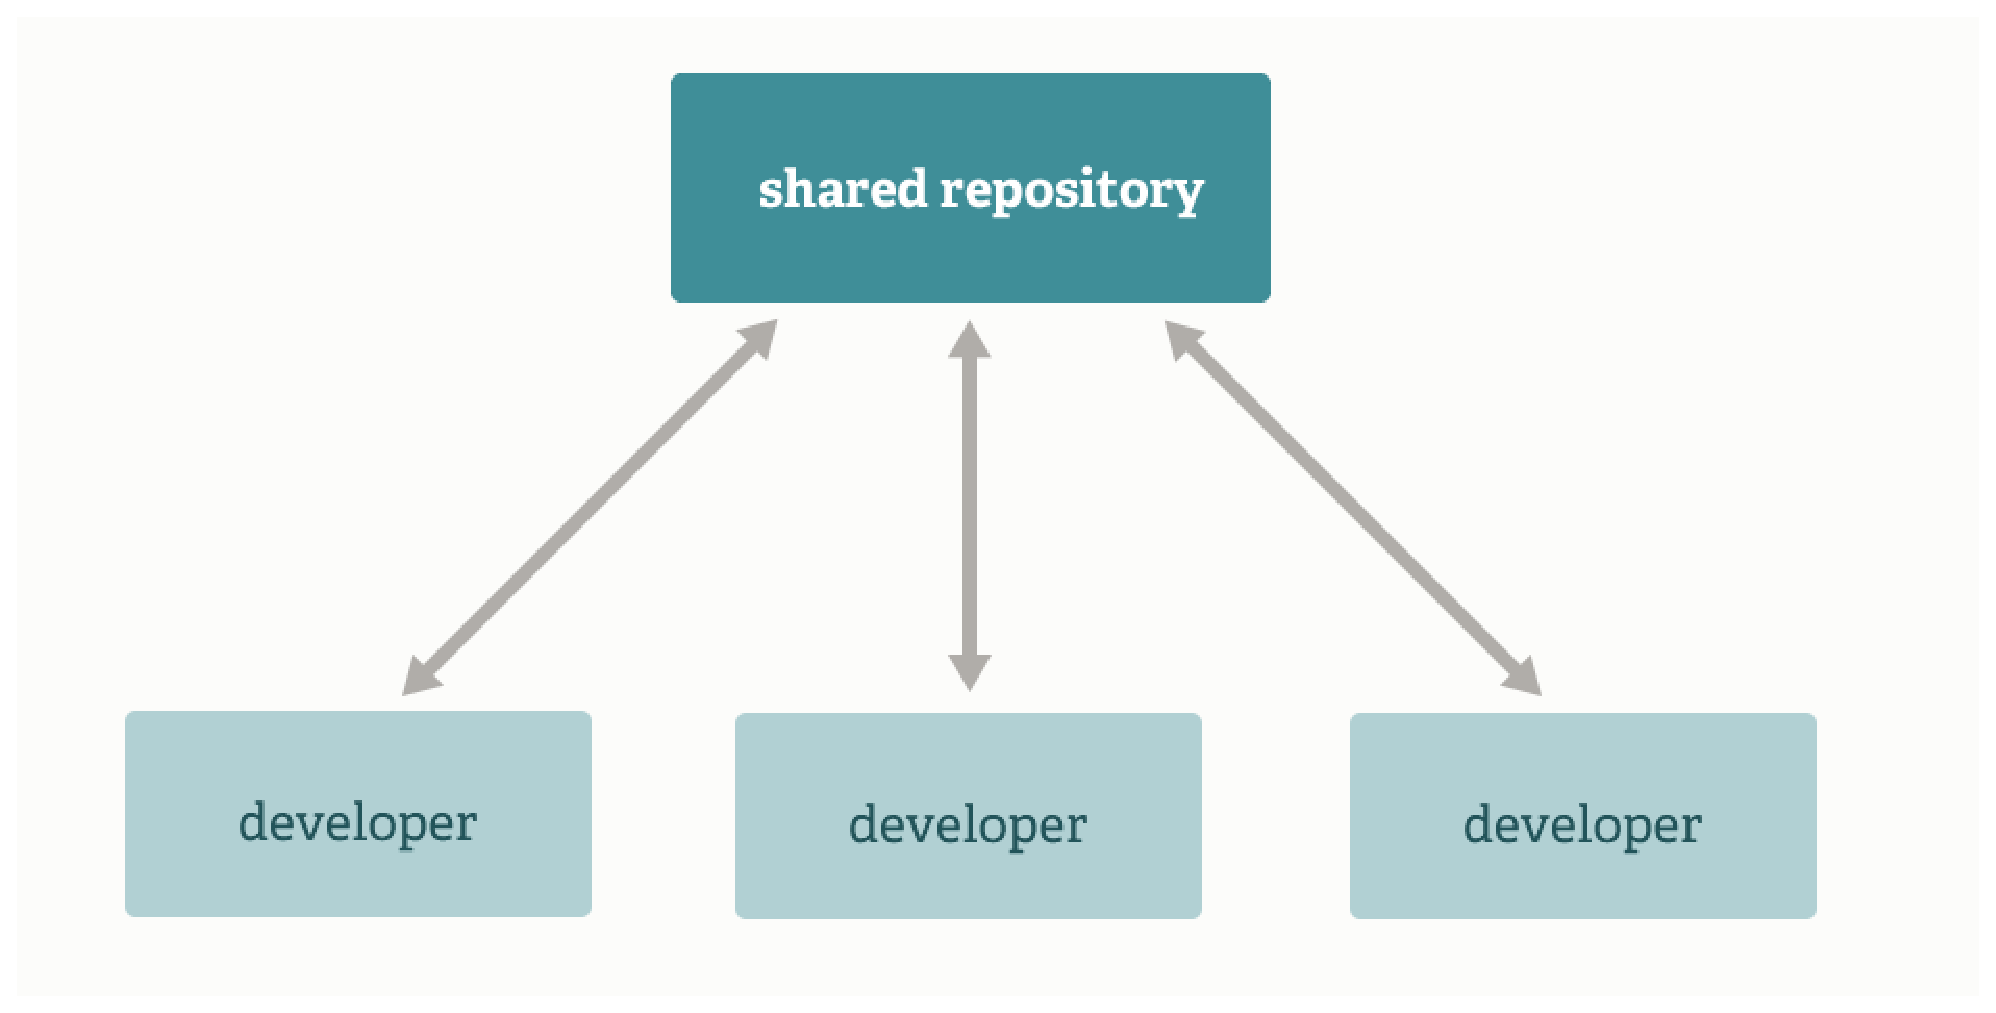
\includegraphics[width=0.5\textwidth]{figuras/git_distribiuted_work.eps}
    \caption{Desenvolvimento distribuído Git}
    Fonte: \cite{git2025}
    \label{fig:git2025}
\end{figure}

\subsection{GitHub}

O GitHub é uma plataforma de hospedagem de código que utiliza o Git como sistema de controle de versão. Além de facilitar a colaboração entre desenvolvedores, o GitHub oferece funcionalidades adicionais, como gerenciamento de projetos e revisão de código. A plataforma é amplamente utilizada para projetos de código aberto e privados, proporcionando um ambiente colaborativo e seguro para o desenvolvimento de software \cite{github2025}.

\subsection{Overleaf e LaTeX}

Overleaf é uma plataforma colaborativa baseada na web que permite a edição de documentos em LaTeX, um sistema de preparação de documentos que utiliza a linguagem de marcação TeX. Overleaf é utilizado em ambientes acadêmicos e profissionais para a criação de artigos científicos, teses e relatórios técnicos, oferecendo ferramentas de colaboração em tempo real e integração com repositórios de controle de versão \cite{overleaf2025}.

\subsection{Google Docs}

O Google Docs é uma aplicação de processamento de texto baseada na web que faz parte do Google Workspace. Oferece funcionalidades de edição colaborativa em tempo real, permitindo que múltiplos usuários trabalhem simultaneamente em um documento. Além disso, o Google Docs integra-se com outras ferramentas do Google, como o Google Drive, facilitando o armazenamento e compartilhamento de documentos \cite{docs2025}.

\subsection{Flutter}

Flutter é um kit de desenvolvimento de código aberto criado pelo Google, utilizado para a criação de aplicativos para dispositivos móveis, web e desktop a partir de uma única base de código. Flutter é compilado nativamente permitindo a criação de interfaces de alta performance, utilizando a linguagem de programação Dart \cite{flutter2025}.

\subsection{Discord}

Discord é uma plataforma de comunicação que oferece serviços de voz, vídeo e texto. A plataforma permite a criação de servidores personalizados, onde os usuários podem organizar canais de comunicação para diferentes tópicos e atividades \cite{discord2025}.

\subsection{Docker}

Docker é uma plataforma de código aberto que automatiza a implantação de aplicações em contêineres de software. Os contêineres permitem que as aplicações sejam executadas de maneira consistente em diferentes ambientes, isolando-as do sistema operacional subjacente. Docker é amplamente utilizado em ambientes de desenvolvimento e produção para garantir a portabilidade e escalabilidade das aplicações \cite{docker2025}.

%\section{Processo Metodológico}

%\subsection{TCC1}

%\section{Simulações}

\section{Arquitetura do Sistema}

Este sistema foi projetado para atender à demanda de tradução de comandos SQL em português para comandos executáveis em um ambiente MySQL, utilizando uma abordagem técnica avançada e uma arquitetura modular que permite escalabilidade, manutenibilidade e extensibilidade.

\subsection{Interface do Usuário}
A interface de usuário foi implementada no framework Flutter, explorando seu sistema declarativo para construir interfaces reativas e de alto desempenho. Ela simula funcionalidades de ferramentas de mercado, como o MySQL Workbench, mas com suporte à inserção de comandos em português. Este front-end é responsável por capturar a entrada do usuário, exibir os resultados traduzidos e lidar com mensagens de erro, utilizando componentes de UI otimizados para acessibilidade e responsividade.

%% Sugestão de imagem: Um mockup da interface de usuário desenvolvida no Flutter, mostrando campos de entrada para comandos em português e uma área para exibição de resultados. Prompt: 'A user interface mockup for a Flutter-based database application, showing input fields for SQL commands in Portuguese and results display.'

Além disso, a arquitetura da interface emprega um padrão MVVM (Model-View-ViewModel), desacoplando a lógica de apresentação da lógica de negócio e permitindo que alterações na interface ou nos fluxos de dados sejam realizadas de maneira independente.

\subsection{Camada de Tradução}
A camada de tradução constitui o núcleo semântico do sistema. Ela foi construída com base em uma lógica de mapeamento semântico-sintático, empregando regras de gramática formal para interpretar e converter comandos SQL em português para o equivalente no padrão ANSI SQL. Para isso, utiliza um banco de dados auxiliar que armazena:

\begin{itemize}
    \item 	extbf{Tokens e Estruturas de Comandos}: Definições de comandos SQL em português mapeados para seus equivalentes em SQL.
    \item 	extbf{Registros de Ambiguidade}: Casos conhecidos de ambiguidades na tradução, tratados por heurísticas específicas.
    \item 	extbf{Logs de Tradução}: Histórico de comandos processados, permitindo otimização futura com base em padrões de uso.
\end{itemize}

\begin{figure}
    \centering
    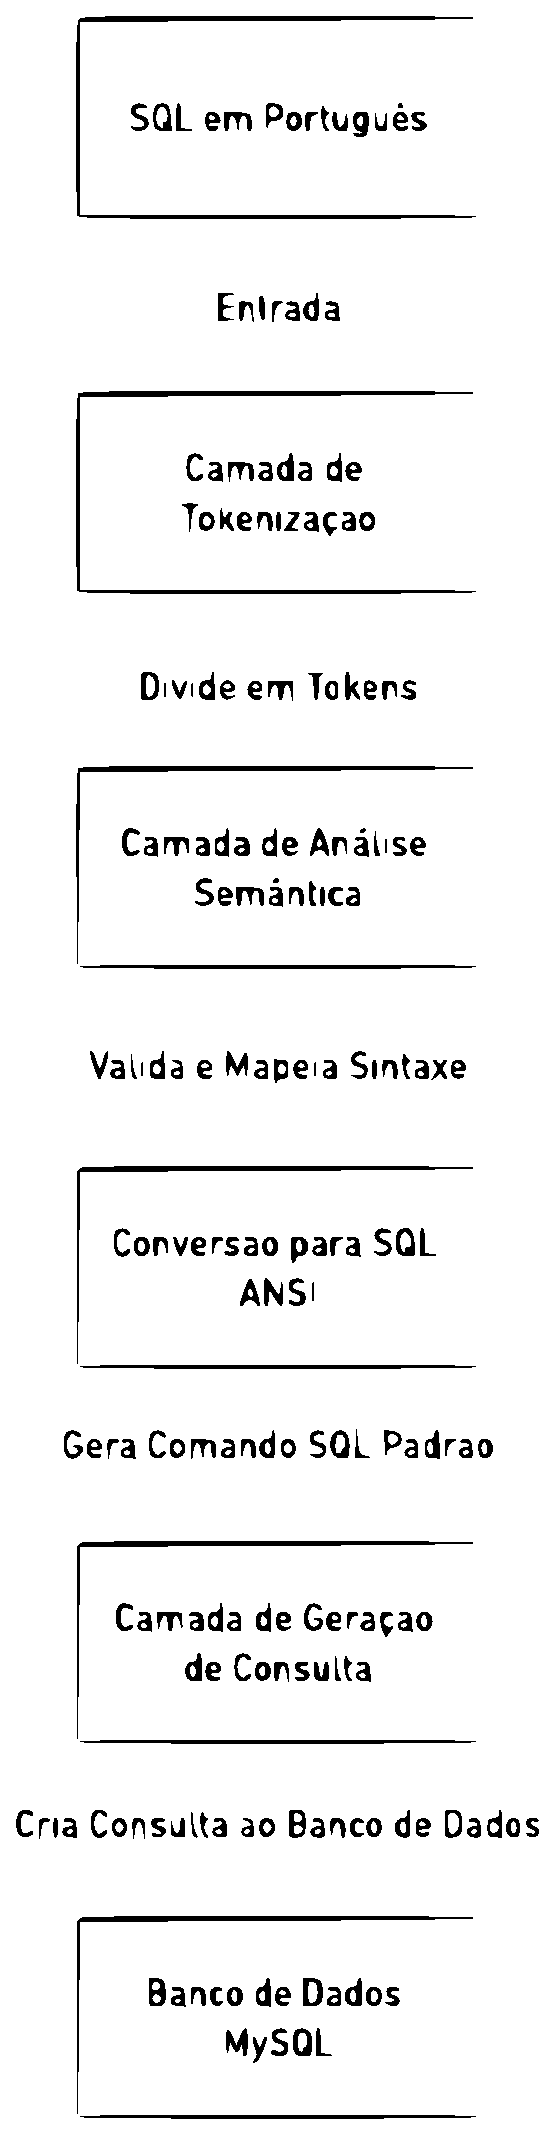
\includegraphics[width=0.3\textwidth]{figuras/traducao.eps}
    \caption{Camada de Integração}
    \label{fig:Camada de tradução}
\end{figure}

A camada também implementa validação semântica para evitar a execução de comandos malformados ou potencialmente inseguros.

\subsection{Banco de Dados MySQL}
O repositório de dados do sistema utiliza uma arquitetura de banco de dados relacional em MySQL, desenhada para desempenho e integridade. O esquema principal é composto pelas seguintes tabelas:

\begin{itemize}
    \item 	extbf{Tabela de Comandos}: Armazena os comandos originais em português e suas correspondências em SQL, organizados por categorias e níveis de complexidade.
    \item 	extbf{Tabela de Respostas}: Contém mensagens padrão do servidor MySQL e suas traduções, otimizadas para consulta por índices compostos.
    \item 	extbf{Tabela de Logs}: Registra operações realizadas pelo sistema, incluindo traduções e execuções, permitindo análise posterior e auditoria.
\end{itemize}

%% Sugestão de imagem: Um diagrama ER (Entidade-Relacionamento) representando as tabelas do banco de dados com seus atributos e relacionamentos. Prompt: 'An entity-relationship diagram for a MySQL database, featuring tables for commands, responses, and logs with their relationships.'

Este design normalizado garante alta eficiência em consultas frequentes e flexibilidade para expansão futura, como suporte a novos idiomas ou bancos de dados alternativos.

\subsection{Camada de Integração}
A camada de integração é implementada como um middleware que gerencia a comunicação entre o front-end e o banco de dados. Ela emprega APIs RESTful para realizar as seguintes operações:

\begin{itemize}
    \item Receber comandos traduzidos da camada de tradução e enviá-los para execução no banco de dados MySQL.
    \item Capturar respostas do banco de dados e encaminhá-las para a camada de tradução de saída.
    \item Implementar mecanismos de autenticação e autorização para garantir a segurança do sistema.
\end{itemize}

\begin{figure}
    \centering
    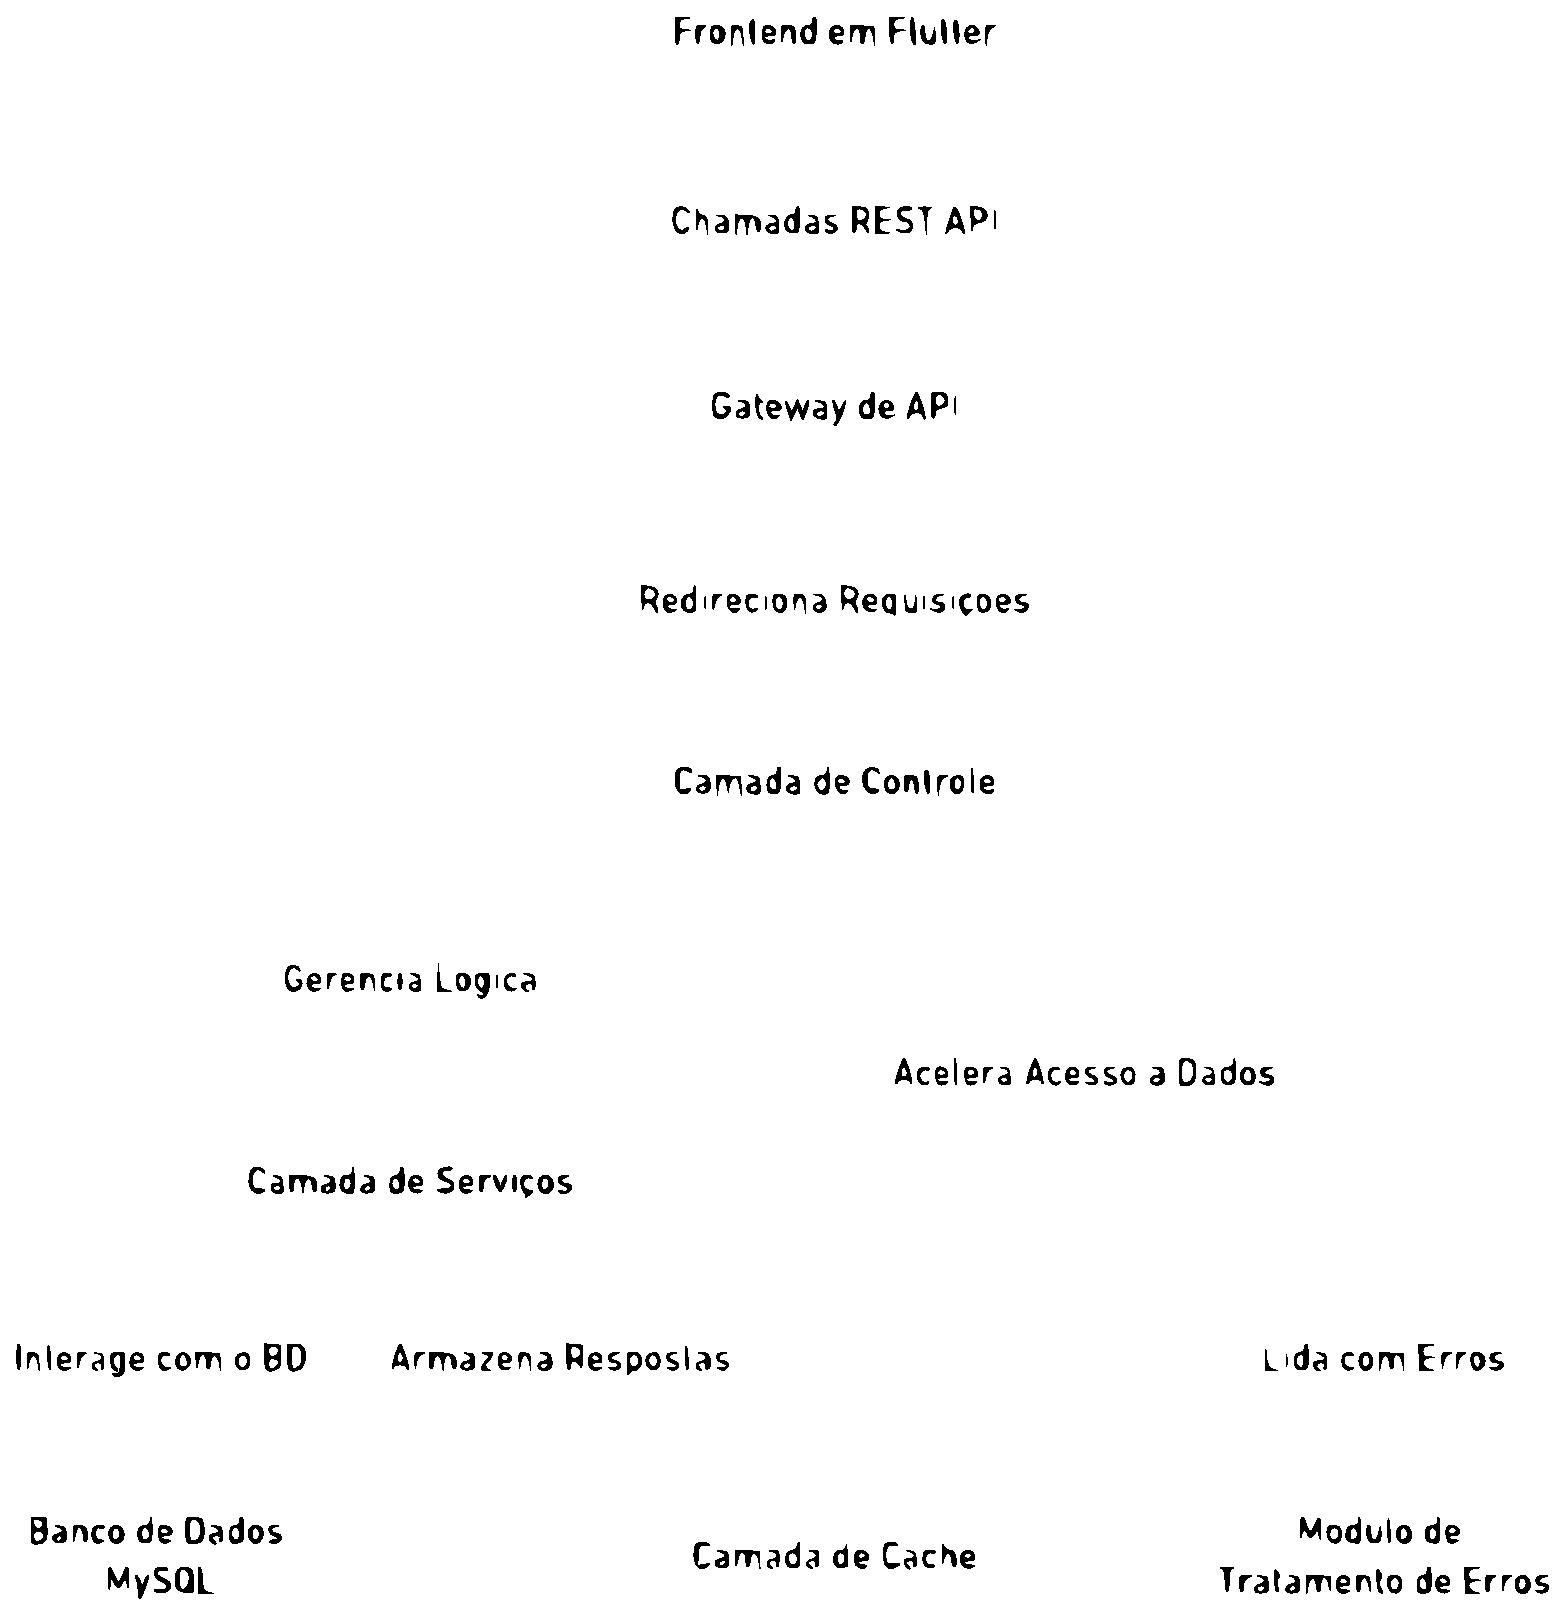
\includegraphics[width=0.5\textwidth]{figuras/mid.eps}
    \caption{Camada de Integração}
    \label{fig:Camada de Integração}
\end{figure}

Além disso, esta camada utiliza técnicas de paralelismo e cacheamento para otimizar o desempenho em cenários de alta concorrência.

\subsection{Fluxo de Dados}
O pipeline de processamento de dados do sistema segue uma sequência bem definida:

\begin{enumerate}
    \item O usuário insere um comando em português na interface do Flutter.
    \item O comando é enviado para a camada de tradução, que utiliza mapeamentos semânticos para convertê-lo em SQL padrão.
    \item A camada de integração transmite o comando traduzido ao servidor MySQL.
    \item O banco de dados executa o comando e retorna uma resposta em inglês.
    \item A camada de tradução converte a resposta para o português, com base no banco de respostas traduzidas.
    \item A interface exibe o resultado final ao usuário.
\end{enumerate}

%% Sugestão de imagem: Um diagrama de fluxo detalhando as etapas do pipeline de processamento de dados. Prompt: 'A flowchart illustrating the data processing pipeline of a SQL translation system, from user input to final output.'

Cada etapa do processo é registrada em logs detalhados, permitindo auditorias e análises de desempenho para identificar gargalos e otimizar o sistema.

\subsection{Modularidade e Escalabilidade}
A arquitetura do sistema é construída com base em princípios de modularidade e desacoplamento. Cada camada funciona como um módulo independente, com interfaces bem definidas, facilitando a substituição ou atualização de componentes individuais. O uso de práticas de design orientado a serviços (SOA) possibilita a extensão para novas funcionalidades sem impacto significativo no funcionamento atual.

Para escalar horizontalmente, o sistema foi projetado para suportar balanceamento de carga na camada de integração, permitindo a distribuição eficiente de requisições entre múltiplos servidores. Adicionalmente, a estrutura de banco de dados pode ser replicada em clusters para suportar alta disponibilidade.

Por fim, a aplicação segue os princípios do design centrado no usuário, priorizando a acessibilidade, desempenho e flexibilidade, garantindo que novos usuários possam aprender conceitos complexos de banco de dados de maneira simplificada, mas tecnicamente precisa.


